\documentclass[11pt]{book}
\usepackage{fontspec}
\setmainfont{TeX Gyre Pagella}
\usepackage[margin=1in]{geometry}
\usepackage{xcolor}
\usepackage{tikz}
\usetikzlibrary{arrows.meta,shapes.geometric,shapes.misc}
\usepackage{amssymb}
\usepackage{enumitem}
\usepackage{titlesec}

\titleformat{\chapter}[display]{\bfseries\Large}{Sproll 08}{0.5em}{\Huge}
\titleformat{\section}{\bfseries\large}{\thesection}{0.6em}{}

\newenvironment{algorithmproc}[1]{\vspace{0.6em}\noindent\rule{\linewidth}{0.6pt}\\[0.2em]\textbf{How to Tell: #1}\\[0.3em]}{\\[0.2em]\noindent\rule{\linewidth}{0.6pt}\vspace{0.6em}}
\newenvironment{practicenow}{\vspace{0.6em}\noindent\rule{\linewidth}{0.6pt}\\[0.2em]\textbf{Practice Now}\\[0.3em]}{\\[0.2em]\noindent\rule{\linewidth}{0.6pt}\vspace{0.6em}}
\newenvironment{exercisebox}[1]{\vspace{0.8em}\noindent\rule{\linewidth}{0.6pt}\\[0.2em]\textbf{Exercises: #1}\\[0.3em]\begin{enumerate}[label=\arabic*., itemsep=0.4em]}{\end{enumerate}\noindent\rule{\linewidth}{0.6pt}\vspace{0.6em}}
\newenvironment{trythis}{\vspace{0.6em}\noindent\rule{\linewidth}{0.6pt}\\[0.2em]\textbf{Try This}\\[0.3em]}{\\[0.2em]\noindent\rule{\linewidth}{0.6pt}\vspace{0.6em}}
\newenvironment{summarybox}{\vspace{0.6em}\noindent\rule{\linewidth}{0.6pt}\\[0.2em]\textbf{What We Learned}\\[0.3em]}{\\[0.2em]\noindent\rule{\linewidth}{0.6pt}\vspace{0.6em}}

\begin{document}
\begin{titlepage}
\centering
\vspace*{1.4in}
{\Huge \textbf{SPROLL 08}}\\[0.5in]
{\huge When Are They Equal?}\\[0.8in]
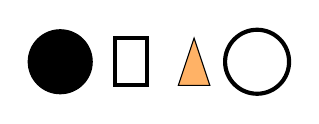
\begin{tikzpicture}
\filldraw[fill=black] (-1.2,0.3) circle (0.16in);
\draw[line width=1.5pt] (-0.5,0) rectangle (-0.1,0.6);
\draw[fill=orange!60] (0.3,0) -- (0.5,0.6) -- (0.7,0) -- cycle;
\draw[line width=1.5pt] (1.3,0.3) circle (0.16in);
\end{tikzpicture}\\[0.8in]
{\Large The Sproll Curriculum}\\[0.2in]
{\large Cycle I: Pops --- Things, Differences, and Counting}
\end{titlepage}

\tableofcontents

\chapter*{Before You Begin}
\addcontentsline{toc}{chapter}{Before You Begin}

Sproll 07 showed that whether two things are ``the same'' depends on which rule you use to look at them. This workbook makes that idea precise and practical: it gives you a clear way to sort and compare things by a stated rule, and shows that changing the rule can completely change which things end up grouped together, even though nothing about the things themselves changed at all.

\chapter{Sorting the Same Objects Two Ways}

\section{Four Shapes, Two Rules}

Here are four shapes: a black circle, an orange square, an orange triangle, and a black circle.

\begin{center}

\begin{tikzpicture}
\filldraw[fill=black] (-1.8,0) circle (0.22in);
\draw[fill=orange!60] (-0.6,-0.22) rectangle (-0.16,0.22);
\draw[fill=orange!60] (0.6,-0.22) -- (0.82,0.22) -- (1.04,-0.22) -- cycle;
\filldraw[fill=black] (2,0) circle (0.22in);
\end{tikzpicture}
\end{center}

Sort them under the rule ``same color.'' You get two piles: the two black circles together, and the orange square with the orange triangle. Now sort the very same four shapes under the rule ``same shape.'' You get three piles: the two circles together, the square alone, and the triangle alone. Nothing about the shapes changed between the two sortings. Only the rule changed, and the groupings that came out of it changed along with it.

\begin{algorithmproc}{Sorting by a Rule}
To sort a group of objects, first state exactly what property the rule cares about (color, shape, size, or anything else). Then place any two objects in the same pile exactly when they agree on that property, and in different piles when they do not. Changing which property the rule cares about can completely change the resulting piles, even with the exact same objects.
\end{algorithmproc}

\begin{practicenow}
Gather a small handful of mixed objects (buttons, coins, crayons, blocks). Sort them once by color and once by size or shape. Confirm you get different groupings from the exact same objects.
\end{practicenow}

\begin{exercisebox}{Section 1.1}
\item Using the four-shape example, explain exactly why ``same color'' and ``same shape'' produce different numbers of piles from the identical four shapes.
\item Sort the letters in your own first name under the rule ``same letter'' and separately under the rule ``vowel or consonant.'' Compare the two groupings.
\item Challenge: can you invent a rule for the four shapes above that would put all four shapes into a single pile together? What property would it have to care about?
\end{exercisebox}

\chapter{Equal Is Relative to a Rule}

\section{Equal Does Not Mean ``Looks Alike''}

It is tempting to think ``equal'' simply means ``looks the same,'' but this workbook wants to sharpen that. Two things are equal under a stated rule exactly when that rule gives the same answer for both of them, whether or not they look alike to the eye. The orange square and orange triangle from the previous section are equal under the color rule (both orange) despite looking nothing alike in shape. The two black circles are equal under both the color rule and the shape rule, which is why they always end up together no matter which of those two rules is used.

\begin{algorithmproc}{Testing Equality}
To check whether two things are equal under a rule, apply the rule separately to each one and compare the results. If the results match, the two things are equal under that rule. If the results differ, they are not equal under that rule, even if they otherwise look very similar.
\end{algorithmproc}

\begin{exercisebox}{Section 2.1}
\item Are a nickel and a dime equal under the rule ``same size,'' the rule ``same value,'' both, or neither? Explain.
\item Give an example of two objects that are equal under a rule about their function or use, despite looking completely different (for example, a wooden spoon and a metal spoon).
\item Challenge: is there a rule under which absolutely everything you own would count as equal to everything else? What would such a rule have to ignore?
\end{exercisebox}

\chapter{Applying This to Histories}

\section{Equal Histories, One More Time}

Recall once more the two histories from Sproll 02 and Sproll 07: circle-then-triangle, and triangle-then-circle. Under the picture rule, applying the rule to each history gives the exact same result, so the two histories are equal under that rule. Under the sequence rule, applying the rule to each history gives two different results, so the two histories are not equal under that rule. This is exactly the same test described in this workbook's algorithm box, just applied to histories instead of shapes.

This also raises a new, harder question. Sproll 05 showed that two separate things can be bound together. Could a whole made of several bound parts ever be equal, under some rule, to the parts it was built from, treated separately? That is not a simple yes-or-no question, and it is exactly where this curriculum goes next.

\begin{summarybox}
Two things are equal under a rule exactly when the rule gives the same result for both of them, regardless of whether they look alike. The same pair of things can be equal under one rule and unequal under another, and both facts can be true at once without contradiction. This applies just as much to histories as it does to shapes, colors, or any other property.
\end{summarybox}

\begin{exercisebox}{Section 3.1}
\item Explain in your own words why ``equal under a rule'' is a more useful idea than a plain, unqualified ``equal.''
\item Take two of your own written sentences that use different words but mean roughly the same thing. Are they equal under a ``same meaning'' rule? Are they equal under an ``exact same words'' rule? Explain both answers.
\item Challenge: can a rule be so loose that literally every pair of things turns out equal under it? Can a rule be so strict that no two distinct things are ever equal under it, even themselves at two different moments in time?
\end{exercisebox}

\chapter*{Looking Ahead}
\addcontentsline{toc}{chapter}{Looking Ahead}

Can several bound parts, considered together, ever be treated as equal to a single whole? And what happens to the parts once they are treated that way, do they disappear, or does some trace of them remain? That is the subject of the next workbook, Sproll 09: Parts With a Past.

\chapter*{For Parents and Teachers}
\addcontentsline{toc}{chapter}{For Parents and Teachers}

This workbook makes precise the rule-relativity of equality introduced informally in Sproll 07, using ordinary sorting as the concrete activity. The key habit this workbook aims to instill is that a bare claim of equality is always shorthand for ``equal under some particular, statable rule,'' and that changing the rule is a legitimate way to change the answer without anyone being wrong. This sets up Sproll 09's treatment of part-whole relationships, where the same rule-relativity is applied to the question of whether a constructed whole is, or is not, equal to the collection of parts it was built from.

\end{document}
